% 2-8 pages, 10pt font
%
% Topics:
%
% * Machine learning based autotuning.
% * Representative benchmarking.
% * Automatic fault tolerance.
% * Run-time adaption.
%

% The following \documentclass options may be useful:
%
% preprint      Remove this option only once the paper is in final form.
% 10pt          To set in 10-point type instead of 9-point.
% 11pt          To set in 11-point type instead of 9-point.
% authoryear    To obtain author/year citation style instead of numeric.
\documentclass[nonatbib,preprint,10pt]{sigplanconf}

%%%%%%%%%%%%%%%%%%%%%%%%%
%% Document and Layout %%
%%%%%%%%%%%%%%%%%%%%%%%%%

% Fix for multiple "No room for a new \dimen" errors.
%
% See: http://tex.stackexchange.com/questions/38607/no-room-for-a-new-dimen
%
\usepackage{etex}

\usepackage[utf8]{inputenc}

% Fix for "'babel/polyglossia' detected but 'csquotes' missing"
% warning. NOTE: Include after inputenc.
%
\usepackage{csquotes}

% Make internal macro definitions accessible,
% e.g. \@title, \@date \@author.
\makeatletter

% Multi-column support.
\usepackage{multicol}

% A useful package which includes macros like \ifdef{}{}{}:
%
\usepackage{etoolbox}

% Uncomment the following line to remove column separation:
%
%\setlength{\columnsep}{5mm}

% Allow user-defined warning and error filters.
%
\usepackage{silence}


%%%%%%%%%%%%%%%%%%%%%
% Table of Contents %
%%%%%%%%%%%%%%%%%%%%%

% % Set chapter and section numbering depth:
% %
% \setcounter{secnumdepth}{2}


%%%%%%%%%%%%%%%%
% Bibliography %
%%%%%%%%%%%%%%%%
\usepackage[%
    backend=biber,
    style=numeric-comp,
    % style=numeric-comp,  % numerical-compressed
    sorting=none,        % nty,nyt,nyvt,anyt,anyvt,ynt,ydnt,none
    sortcites=true,      % sort \cite{b a d c}: true,false
    block=none,          % space between blocks: none,space,par,nbpar,ragged
    indexing=false,      % indexing options: true,false,cite,bib
    citereset=none,      % don't reset cites
    isbn=false,          % print ISBN?
    url=true,            % print URL?
    doi=false,           % print DOI?
    natbib=true,         % natbib compatability
  ]{biblatex}

% % Filter annoying and unavoidable biblatex warning:
\WarningFilter{biblatex}{Patching footnotes failed}

% Reduce the font size of the bibliography:
% \renewcommand{\bibfont}{\normalfont\scriptsize}

% Determine which BibTeX file to use:
%
% If available, use my Mendeley BibTex library, located in the home
% directory. Note that this is a relative path and will break if
% either this file or the BibTex library are moved. If the library is
% not present, use the local refs.bib file.
\newcommand{\BibResourceGlobal}{../../library.bib}
\newcommand{\BibResourceLocal}{refs.bib}

\IfFileExists{\BibResourceGlobal}
  {\newcommand{\BibResource}{\BibResourceGlobal}}
  {\newcommand{\BibResource}{\BibResourceLocal}}

\addbibresource{\BibResource}


%%%%%%%%%%%%%%
% Appendices %
%%%%%%%%%%%%%%

% Appendix package. Documentation:
%
%  http://mirror.ox.ac.uk/sites/ctan.org/macros/latex/contrib/appendix/appendix.pdf
%
% Package options:
%
% toc      - Put a header (e.g., `Appendices') into the Table of Contents
%            (the ToC) before listing the appendices. (This is done by
%            calling the \addappheadtotoc command.)
% page     - Puts a title (e.g., `Appendices') into the document at the
%            point where the appendices environment is begun. (This is
%            done by calling the \appendixpage command.)
% title    - Adds a name (e.g., `Appendix') before each appendix title in
%            the body of the document. The name is given by the value
%            of \appendixname. Note that this is the default behaviour
%            for classes that have chapters.
% titletoc - Adds a name (e.g., `Appendix') before each appendix listed
%            in the ToC. The name is given by the value
%            of \appendixname.
% header   - Adds a name (e.g., `Appendix') before each appendix in page
%            headers.  The name is given by the value
%            of \appendixname. Note that this is the default behaviour
%            for classes that have chapters.
\usepackage[title, titletoc]{appendix}


%%%%%%%%%%%%%%%%%%%%%%%%%%%%%%%%%%%%%
%% Figures, footnotes and listings %%
%%%%%%%%%%%%%%%%%%%%%%%%%%%%%%%%%%%%%

%\usepackage{float}
%\restylefloat{figure}

% Use bold ``(Figure|Table|Listing)'' caption text.
%\usepackage[margin=1cm]{caption}

% Set the font for captions.
% \renewcommand{\captionfont}{\small}
% Set the font for caption labels.
% \renewcommand{\captionlabelfont}{\footnotesize\bf}

% Use arabic numbers for footnote.
%\renewcommand{\thefootnote}{\arabic{footnote}}

% Ensure that footnotes always appear at the bottom of pages.
%\usepackage[bottom]{footmisc}

% Reset the footnote counter on every page.
%\usepackage{perpage}
%\MakePerPage{footnote}

% Pre-requisites for rendering upquotes in listings package.
\usepackage[T1]{fontenc}
\usepackage{lmodern}
\usepackage{textcomp}

% Pseudo-code listings.
\usepackage{algorithm}
\usepackage{algpseudocode}
\newcommand{\Break}{\State \textbf{break} }
\algblockdefx[Loop]{Loop}{EndLoop}[1][]{\textbf{Loop} #1}{\textbf{End
    Loop}}

\algrenewcommand\ALG@beginalgorithmic{\footnotesize}

% Code listings.
\usepackage{listings}

% Set \ttfamily to use courier fonts.
%
% See: http://tex.stackexchange.com/a/33686
%
\usepackage{courier}

\lstset{frame=bt,                    % Add top and bottom frame lines
        breaklines=true,             % Force line wrapping
        captionpos=b,                % Place caption below listing
        numbers=left,                % Add left-side line numbers
        basicstyle=\scriptsize\ttfamily, % Set font size and type
        showstringspaces=false,      % Don't show visible whitespace
        numberstyle=\tiny,
        upquote=true,                % Use upright quotes, not curly
        commentstyle=\bfseries}      % Embolden comments

% Use (*@ @*) to escape LaTeX commands within listings.
\lstset{escapeinside={(*@}{@*)}}

% Add 10pt space between chapters in TOC listings entries:
%\let\Chapter\chapter
%\def\chapter{\addtocontents{lol}{\protect\addvspace{10pt}}\Chapter}


%%%%%%%%%%%%%%%%%%%%%%%%
%% Graphics and maths %%
%%%%%%%%%%%%%%%%%%%%%%%%
\usepackage{amsmath}

% Vector notation, e.g. \vv{x}:
%
\usepackage{esvect}

% Additional amsmath symbols, see:
%
% http://texblog.org/2007/08/27/number-sets-prime-natural-integer-rational-real-and-complex-in-latex/
%
\usepackage{amsfonts}
\usepackage{amssymb}

\usepackage{graphicx}
\usepackage{mathtools}
\usepackage{tikz}
\usepackage{tikz-qtree}

% Provide bold font face in maths.
\usepackage{bm}

\usepackage{subcaption}
\expandafter\def\csname ver@subfig.sty\endcsname{}

% Define an 'myalignat' command which behave as 'alignat' without the
% vertical top and bottom padding. See:
%     http://www.latex-community.org/forum/viewtopic.php?f=5&t=1890
\newenvironment{myalignat}[1]{%
  \setlength{\abovedisplayskip}{-.7\baselineskip}%
  \setlength{\abovedisplayshortskip}{\abovedisplayskip}%
  \start@align\z@\st@rredtrue#1
}%
{\endalign}

% Define additional operators:
\DeclareMathOperator*{\argmin}{arg\,min}
\DeclareMathOperator*{\argmax}{arg\,max}

\DeclareMathOperator*{\gain}{Gain}

% Skeleton operators.
\DeclareMathOperator*{\map}{Map}
\DeclareMathOperator*{\reduce}{Reduce}
\DeclareMathOperator*{\scan}{Scan}
\DeclareMathOperator*{\stencil}{Stencil}
\DeclareMathOperator*{\zip}{Zip}
\DeclareMathOperator*{\allpairs}{All\,Pairs}

% Maths plots using pgfplots, see:
%
%     http://pgfplots.sourceforge.net/pgfplots.pdf
%
\usepackage{pgfplots}

% Disable compatability mode.
%
\pgfplotsset{compat=1.12}

% Gantt charts using pgfgantt, see:
%
%     http://www.ctan.org/pkg/pgfgantt
%
\usepackage{pgfgantt}

% Fix milestone aspect ratio by defining a custom element.
\newganttchartelement*{mymilestone}{
  mymilestone/.style={
    shape=diamond,
    inner sep=2pt,
    draw=black,
    top color=black,
    bottom color=black,
  }
}

% Tikz flowchart configuration.
\usetikzlibrary{shapes,arrows,shadows,fit,backgrounds}
\tikzstyle{decision} = [diamond,
                        draw,
                        text width=4.5em,
                        text badly centered,
                        node distance=3cm,
                        inner sep=0pt]
\tikzstyle{block}    = [rectangle,
                        draw,
                        text width=5em,
                        text centered,
                        node distance=3cm,
                        minimum height=4em,
                        inner sep=.2cm]
\tikzstyle{line}     = [draw, -latex']

% Add dirtree picture style, see:
%
%     http://tex.stackexchange.com/a/34268
%
\newcount\dirtree@lvl
\newcount\dirtree@plvl
\newcount\dirtree@clvl
\def\dirtree@growth{%
  \ifnum\tikznumberofcurrentchild=1\relax
    \global\advance\dirtree@plvl by 1
    \expandafter\xdef\csname dirtree@p@\the\dirtree@plvl\endcsname{\the\dirtree@lvl}
  \fi
  \global\advance\dirtree@lvl by 1\relax
  \dirtree@clvl=\dirtree@lvl
  \advance\dirtree@clvl by -\csname dirtree@p@\the\dirtree@plvl\endcsname
  \pgf@xa=0.33cm\relax
  \pgf@ya=-\baselineskip\relax
  \pgf@ya=\dirtree@clvl\pgf@ya
  \pgftransformshift{\pgfqpoint{\the\pgf@xa}{\the\pgf@ya}}%
  \ifnum\tikznumberofcurrentchild=\tikznumberofchildren
    \global\advance\dirtree@plvl by -1
  \fi
}
\tikzset{
  dirtree/.style={
    growth function=\dirtree@growth,
    every node/.style={anchor=north},
    every child node/.style={anchor=west},
    edge from parent path={(\tikzparentnode\tikzparentanchor) |- (\tikzchildnode\tikzchildanchor)}
  }
}

% UML sequence diagram macros, see:
%
%     https://code.google.com/p/pgf-umlsd/
%
% Options:
%
%     underline - Underline object names
%
\usepackage[underline=false]{pgf-umlsd}

% Support for SVG graphics.
%
% NOTE that you must pass the "--shell-escape" argument to pdflatex to
% compile. NOTE also that images *MUST* be placed within the graphics
% path.
\usepackage{svg}
\graphicspath{{img/}}

%%%%%%%%%%%%%%%%%%%%%%
%% Tables and lists %%
%%%%%%%%%%%%%%%%%%%%%%

% Required to use labm8 exported tables.
%
\usepackage{booktabs}

% Required for full page-width tables.
\usepackage{tabularx}

%\usepackage{enumitem}
%\setenumerate{itemsep=0pt}

% Use no left margin for lists:
%\setlist{leftmargin=*}

\usepackage{longtable}

% Define column types L, C, R with known text justification and fixed
% widths:
\usepackage{array}
\newcolumntype{L}[1]{>{\raggedright\let\newline\\\arraybackslash\hspace{0pt}}m{#1}}
\newcolumntype{C}[1]{>{\centering\let\newline\\\arraybackslash\hspace{0pt}}m{#1}}
\newcolumntype{R}[1]{>{\raggedleft\let\newline\\\arraybackslash\hspace{0pt}}m{#1}}


%%%%%%%%%%%%%%%%%%%%%%%%%%%%%
%% Typesetting and symbols %%
%%%%%%%%%%%%%%%%%%%%%%%%%%%%%

% Adjustable font sizes in \Verbatim{}
\usepackage{fancyvrb}

%\usepackage{titlesec}
% Set section and paragraph heading fonts:
%\titleformat*{\section}{\Large\bfseries}
%\titleformat*{\subsection}{\normalsize\bfseries}
%\titleformat*{\subsubsection}{\normalsize}
%\titleformat*{\paragraph}{\large\bfseries}
%\titleformat*{\subparagraph}{\large\bfseries}

% Set section heading margins. Usage:
% \titlespacing*{<command>}{<left>}{<before>}{<after>}
%\titlespacing*{\section}{0pt}{.6em}{.3em}
%\titlespacing*{\subsection}{0pt}{.6em}{.2em}

% Set paragraph indentation size. Default is 15pt.
%\setlength{\parindent}{10pt}

% The line spacing can be globally set using \linespread:
%
% \linespread{1.2}

% Add a command \hr{} which will draw a horizontal rule the width of
% the text.
%
\newcommand{\hr}{\noindent\makebox[\linewidth]{\rule{\textwidth}{0.2pt}}}

% Add a command \br{} which will create a horizontal space of exactly
% one line height.
%
\newcommand{\br}{\hspace{\baselineskip}}

% Define a command to allow word breaking.
\newcommand*\wrapletters[1]{\wr@pletters#1\@nil}
\def\wr@pletters#1#2\@nil{#1\allowbreak\if&#2&\else\wr@pletters#2\@nil\fi}

% Define a command to create centred page titles.
\newcommand{\centredtitle}[1]{
  \begin{center}
    \large
    \vspace{0.9cm}
    \textbf{#1}
  \end{center}}

% Support hyperlinks using the \hyperref, \url and \href
% macros. Usage:
%
%    \hyperref[label_name]{''link text''}
%
%    \url{<my_url>}
%
%    \href{<my_url>}{<description>}
%
\usepackage{hyperref}

% Disable colored borders of links, cross-references etc in PDF output
\hypersetup{pdfborder={0 0 0}}

% Provide generic commands \degree, \celsius, \perthousand, \micro
% and \ohm which work both in text and maths mode.
\usepackage{gensymb}

%%%%%%%%%%%%%%%%%%%%%%%%%%%%%%%%%
%% Placeholder text generation %%
%%%%%%%%%%%%%%%%%%%%%%%%%%%%%%%%%

% Use either \blindtext or \libpsum to generate placeholder text. Also
% note the macros \blinditemize, \blindenumerate, \blinddescription.
\usepackage[english]{babel}
\usepackage{blindtext}
\usepackage{lipsum}


\begin{document}

\special{papersize=8.5in,11in}
\setlength{\pdfpageheight}{\paperheight}
\setlength{\pdfpagewidth}{\paperwidth}

\conferenceinfo{ADAPT '16}{Month d--d, 20yy, City, ST, Country}
\copyrightyear{2016}
\copyrightdata{978-1-nnnn-nnnn-n/yy/mm}
\doi{nnnnnnn.nnnnnnn}

% Uncomment one of the following two, if you are not going for the
% traditional copyright transfer agreement.

%\exclusivelicense                % ACM gets exclusive license to publish,
                                  % you retain copyright

%\permissiontopublish             % ACM gets nonexclusive license to publish
                                  % (paid open-access papers,
                                  % short abstracts)

% \titlebanner{banner above paper title}        % These are ignored unless
\preprintfooter{ADAPT workshop '16}   % 'preprint' option specified.

% \title{Autotuning Stencil Codes using Synthetic Benchmarks}
% \title{Autotuning OpenCL Workgroup Sizes for Stencil Codes}
% \title{Machine learning for OpenCL Workgroup Sizes of Stencil Codes}
% \title{Machine learning for OpenCL Workgroup Sizes of Stencil Codes}
% \title{Methods for Autotuning Workgroup Size of OpenCL Stencil Codes}
\title{Autotuning OpenCL Workgroup Size for Stencil Patterns}

% Comparison of multiple approaches to autotuning stencil patterns:
%
% * Compare classifiers with regressors
% * Compare synthetic vs real training

% \subtitle{Subtitle Text, if any}

\authorinfo{Chris Cummins\and Pavlos Petoumenos\and Hugh Leather}
           {University of Edinburgh}
           {c.cummins@ed.ac.uk,\{ppetoume,hleather\}@inf.ed.ac.uk}

\maketitle

\begin{abstract}
  Selecting the appropriate workgroup size for OpenCL kernels requires
  knowledge of the underlying hardware, the data being operated on,
  and properties of the kernel. This makes portable performance tuning
  a difficult task, and simple heuristics and statically chosen values
  fail to exploit the available performance. To address this, we
  propose the use of machine learning-enabled autotuning to predict
  workgroup sizes for stencil patterns on CPUs and GPUs.

  We present three methodologies for predicting workgroup sizes. The
  first, using classifiers to select the optimal workgroup size. The
  second and third proposed methodologies employ the novel use of
  regressors for performing classification by predicting the runtime
  of kernels and relative performance of different workgroup sizes,
  respectively. In an empirical evaluation of 429 combinations of
  architecture, kernel, and dataset, our methods provides a median
  $3.79\times$ speedup over the best possible performance which can be
  achieved without autotuning, achieving 94\% of the available
  performance. % We compare the impact that selection of machine
  % learning models and autotuning approach has on performance.
\end{abstract}

% \category{CR-number}{subcategory}{third-level}

% % general terms are not compulsory anymore,
% % you may leave them out
% % \terms
% % term1, term2

% \keywords
% keyword1, keyword2

\section{Introduction}\label{sec:introduction}

Stencil codes have a variety of computationally expensive uses from
fluid dynamics to quantum mechanics. Efficient, tuned stencil
implementations are highly sought after, with early work in
\citeyear{Bolz2003} by \citeauthor{Bolz2003} demonstrating the
capability of GPUs for massively parallel stencil
operations~\cite{Bolz2003}. Since then, the standardisation of OpenCL
has introduced greater programmability of heterogeneous devices by
providing a vendor-independent layer of abstraction for data parallel
programming of CPUs, GPUs, DSPs, and other
devices~\cite{Stone2010}.

%This allows the development of high level
% patterns to simplify parallel programming by providing generic

 However, achieving portable performance of
OpenCL programs is a hard task --- such programs are sensitive to
properties of the underlying hardware, to the program being executed,
and even to the \emph{dataset} that is operated upon. This forces
developers to laboriously hand tune performance on a per-program
basis, since simple heuristics fail to exploit the available
performance.

% Higher level programming abstractions aim to address this issue by
% simplifying the programmability to challenge, raising the level of
% abstraction above

In this paper, we implement machine learning-enabled autotuning for
one such optimisation parameter of OpenCL programs --- that of
workgroup size selection. This autotuning is applied to stencil codes
using the SkelCL Algorithmic Skeleton library.

% SkelCL is a C++ framework which allows users to easily harness the
% power of CPUs and multi-GPU systems. The

Introduced in~\cite{Steuwer2011}, SkelCL is an object oriented C++
library that provides OpenCL implementations of data parallel
algorithmic skeletons for heterogeneous parallelism using CPUs or
multi-GPUs. SkelCL addresses the parallel programmability challenge by
allowing users to easily harness the power of GPUs and CPUs for data
parallel computing.

Stencil workgroup sizes presents a two dimensional parameter space,
consisting of a number of rows and columns. It is constrained by
properties of both the stencil code and underlying architecture. The
optimisation space presented by the workgroup size of OpenCL kernels
is large, complex, and non-linear. Successfully applying machine
learning to such a space requires plentiful training data, the careful
selection of features, and an appropriate classification approach.


\section{The SkelCL Stencil Skeleton}

\begin{figure}
\centering
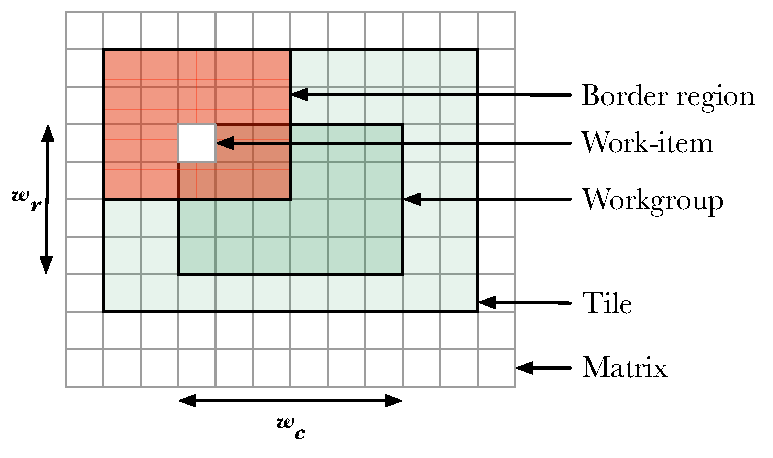
\includegraphics[width=.75\columnwidth]{img/stencil}
\caption[Stencil border region]{%
  The components of a stencil: an input matrix is decomposed into
  workgroups, consisting of $w_r \times w_c$ elements. Each element is
  mapped to a work-item. Each work-item operates its corresponding
  element and a surrounding border region $S$, consisting of the four
  independent components describing the number of elements north
  $S_n$, east $S_e$, west $S_w$, and south $S_s$ (in this example, 1
  element to the south, and 2 elements in all other directions). Each
  tile is allocated in local memory for fast access of repeated read
  operations.%
}
\label{fig:stencil-shape}
\end{figure}

SkelCL provides a stencil skeleton in which a user-provided
\emph{customising function} is applied to each element of a 2D
matrix~\cite{Breuer2014a}. The value of each element is updated based
on its current value and the value of one or more neighbouring
elements, called the \emph{border region}. The border region is
described by a \emph{stencil shape}, which defines an $i \times j$
rectangular region about each cell which is used to update the cell
value. Stencil shapes may be asymmetrical, and are defined in terms of
the number of cells in the border region to the north, east, south,
and west of each cell, shown in Figure~\ref{fig:stencil-shape}. Where
elements of a border region which fall outside of the matrix bounds,
values are substituted from either a predefined padding value, or the
value of the nearest cell within the matrix, depending on user
preference.

Each element of a stencil input matrix is mapped to a single OpenCL
work-item; and this collection of work-items is then divided into
\emph{workgroups} for execution on the target hardware. Each work-item
reads the value of the corresponding element and the surrounding
elements defined by the border region. Since the border regions of
neighbouring elements overlap, the value of all elements within a
workgroup are stored in a \emph{tile}, allocated as a contiguous block
of local memory. As local memory access times are much shorter than
that of global memory, this greatly reduces the latency of the border
region reads performed by each work-item. Changing the workgroup size
thus affects the amount of local memory required for each workgroup,
which in turn affects the number of workgroups which may be
simultaneously active. So while the user defines the size, type, and
border region of the of the grid being operated upon, it is the
responsibility of the SkelCL stencil implementation to select an
appropriate workgroup size to use.


\section{Autotuning Workgroup Size}

Selecting the appropriate workgroup size for a kernel depends on the
properties of the kernel itself, underlying architecture, and
dataset. For a given \emph{scenario} (that is, a particular
combination of kernel, architecture, and dataset), the goal of this
work is to harness machine learning to \emph{predict} a performant
workgroup size to use, based on some prior knowledge of the
performance of workgroup sizes for other scenarios. The space of
possible workgroup sizes $W$ is constrained by properties of both the
architecture and kernel.

\subsection{Constraints}

Each OpenCL device imposes a maximum workgroup size which can be
statically checked through the OpenCL Device API. This constraint
reflects architectural limitations of how code is mapped to the
underlying execution hardware. Typical values are powers of two, e.g.\
1024, 4096, 8192. Additionally, kernels enforce a maximum workgroup
size. This value can be queries at runtime once a program has been
compiled for a specific execution device. Factors which affect a
kernel's maximum workgroup size include the number of registers
required for a kernel, and the available number of SIMD execution
units for each type of instructions in a kernel.

While in theory, any workgroup size which satisfies the device and
kernel workgroup size should provide a functioning program, in
practise we did not find this to be the case. As such, we define
\emph{refused parameters} as workgroup sizes which satisfy the kernel
and architectural constraints, yet cause a
\texttt{CL\_OUT\_OF\_RESOURCES} error to be thrown when the kernel is
enqueued. Note that in many OpenCL implementations, this error type
acts as a generic placeholder and may not necessarily indicate that
the underlying cause of the error was due to finite resources
constraints. Further discussion on the possible causes and effects of
refused parameters is contained in Section~XXX, but for now we use the
concept of refused parameters to formalise the constraints on the
workgroup size space. We define a \emph{legal} workgroup size as one
satisfies the architectural and kernel constraints of a given
scenario, and is not refused. The subset of all possible workgroup
sizes $W_{legal}(s) \subset W$ that are legal is then:
%
\begin{equation}
  \footnotesize
  W_{legal}(s) = \left\{w | w \in W, w < W_{\max}(s) \right\} - W_{refused}(s)
\end{equation}
%
Where $W_{\max}(s)$ can be determined at runtime prior to the kernels
execution, but the set $W_{refused}(s)$ can only be discovered
emergently.


%\subsection{Optimisation Target}
%
% %
% We can quantify the performance $p(s,w)$ of a particular workgroup
% size relative to the oracle, within the range $0 \le p(s,w) \le 1$,
% using $p(s,w) = \frac{t(s,\Omega(s)}{t(s,w)}$. Across a set of
% scenarios $S$, the average performance $\bar{p}(w)$ of a workgroup
% size is calculated using the geometric mean of performances:
% % Across the set of all scenarios $S$, the average performance
% % $\bar{p}(w)$ of the workgroup size is found using the geometric mean
% % of performances:
% %
% % \begin{align}
% %   p(s,w) &= \frac{t(s,\Omega(s)}{t(s,w)}\\
% %   \bar{p}(w) &=
% %   \left(
% %     \prod_{s \in S} p(s,w))
% %   \right)^{1/|S|}
% % \end{align}
% \begin{equation}
%   \bar{p}(w) =
%   \left(
%     \prod_{s \in S} p(s,w))
%   \right)^{1/|S|}
% \end{equation}
% %
% The \emph{baseline} workgroup size is the value which provides the
% best average case performance across all scenarios. Such a baseline
% value represents the \emph{best} possible performance which can be
% achieved using a single, statically chosen workgroup size. By defining
% $W_{safe} \in W$ as the intersection of legal workgroup sizes, the
% baseline workgroup size $\bar{w}$ can be found using:
% %
% \begin{align}
% W_{safe} &= \cap \left\{ W_{legal}(s) | s \in S \right\}\\
% \bar{w} &= \argmax_{w \in W_{safe}} \bar{p}(w)
% \end{align}


\subsection{Stencil Features}

Since properties of the architecture, program, and dataset all
contribute to the performance of a workgroup size, the success of a
machine learning system depends on the ability to translate these
properties into meaningful explanatory variables ---
\emph{features}. For each scenario, 102 features are extracted
describing the architecture, kernel, and dataset.

Architecture features are extracted using the OpenCL Device API to
query properties such as the size of local memory, maximum work group
size, and number of compute units. For kernel feature, the source code
for a stencil kernel is compiled to LLVM IR bitcode, and a statistics
pass is used to obtain static counts for each type of instruction
present in the kernel, as well as the total number of
instructions. The instruction counts for each type are divided by the
total number of instructions to produce a \emph{density} of
instruction for that type. Examples include total static instruction
count, ratio of instructions per type, and ratio of basic blocks per
instruction. Dataset features include the input and output data types,
and the 2D matrix dimensions.


\subsection{Training Data}\label{subsec:training}

Training data are collected by measuring the runtimes of stencil
programs using different workgroup sizes. These stencil programs are
generated synthetically using a parameterised template substitution
engine. A stencil template is parameterised first by stencil shape
(one parameter for each of the four directions), input and output data
types (either integers, or single or double precision floating
points), and \emph{complexity} --- a simple boolean metric for
indicating the desired number of memory accesses and instructions per
iteration, reflecting the relatively bi-modal nature of stencil codes,
either compute intensive (e.g.\ finite difference time domain and
other PDE solvers), or lightweight (e.g.\ Game of Life and Gaussian
blur).


\section{Machine Learning Methods}

The challenge is to design a system which, given a set of prior
observations of the empirical performance of stencil codes with
different workgroup sizes, predicts workgroup sizes for \emph{unseen}
scenarios which maximise the performance. This section presents three
methods for achieving this goal.


\subsection{Predicting Oracle Workgroup Size}

\begin{algorithm}[t]
\begin{algorithmic}[1]
\Require scenario $s$, classifier $C(x)$
\Ensure workgroup size $w$

\Procedure{Baseline}{s}
% \Comment Select the best $w$ from $W_{safe}$.
\State $w \leftarrow C(f(s))$
\If{$w \in W_{legal}(s)$}
    \State \textbf{return} $w$
\Else
  \State \textbf{return} $\underset{w \in W_{safe}}{\argmax}
\left(
  \prod_{s \in S_{training}} p(s, w)
\right)^{1/|S_{training}|}$
\EndIf
\EndProcedure
\item[] % line break

\Procedure{Random}{s}
% \Comment Select a random workgroup size.
\State $w \leftarrow C(f(s))$
\While{$w \not\in W_{legal}(s)$}
  \State $W \leftarrow \left\{ w | w < W_{max}(s), w \not\in W_{refused}(s) \right\}$
  \State $w \leftarrow $ random selection $w \in W$
\EndWhile
\State \textbf{return} $w$
\EndProcedure
\item[] % line break

\Procedure{NearestNeighbour}{s}
% \Comment Select the closest workgroup size to prediction.
\State $w \leftarrow C(f(s))$
\While{$w \not\in W_{legal}(s)$}
  \State $d_{min} \leftarrow \infty$
  \State $w_{closest} \leftarrow \text{null}$
  \For{$c \in \left\{ w | w < W_{\max}(s), w \not\in W_{refused}(s) \right\}$}
    \State $d \leftarrow \sqrt{\left(c_r - w_r\right)^2 + \left(c_c - w_c\right)^2}$
    \If{$d < d_{min}$}
      \State $d_{min} \leftarrow d$
      \State $w_{closest} \leftarrow c$
    \EndIf
  \EndFor
  \State $w \leftarrow w_{closest}$
\EndWhile
\State \textbf{return} $w$
\EndProcedure
\end{algorithmic}
\caption{Predicting using classifiers}
\label{alg:autotune-classification}
\end{algorithm}

The first approach to predicting workgroup sizes is to consider the
set of possible workgroup sizes as a hypothesis space and to use a
classifier to predict, for a given set of features, the \emph{oracle}
workgroup size $\Omega(s)$, which is the workgroup size which provides
the lowest mean runtime $t(s,w)$:
%
\begin{equation}
  \Omega(s) = \argmin_{w \in W_{legal}(s)} t(s,w)
\end{equation}
%
Training data consists of pairs of features $f(s)$ labelled with their
oracle workgroup size for a set of training scenarios $S_{training}$:
%
\begin{equation}
  D_{training} = \left\{ \left(f(s), \Omega(s)\right) | s \in S_{training} \right\}
\end{equation}
%
After training, the classifier predicts workgroup sizes for unseen
scenarios from the set of oracle workgroup sizes from the training
set. This is a common and intuitive approach to autotuning, in that
machine learning is used to predict the best parameter value for a new
scenario based on what were the best parameter values for previous
scenarios. However, given the constrained space of workgroup sizes,
this presents a problem that after training, there is no guarantee
that the set of workgroup sizes which may be predicted is within the
set of legal workgroup sizes for future scenarios:
%
\begin{equation}
  \left\{ \Omega(s) | s \in S_{training} \right\} \nsubseteq \bigcup_{\forall s \in S_{future}} W_{legal}(s)
\end{equation}
%
This results in a classifier which may predict workgroup sizes that
are not legal for scenarios, either because it exceeds $W_{\max}(s)$,
or because the parameter is refused, $w \in W_{refused}(s)$. For these
cases, we evaluate the effectiveness of three \emph{fallback
  strategies} to select a legal workgroup size:
%
\begin{enumerate}
\item \emph{Baseline} --- select the workgroup size which is known to
  be safe $w < W_{safe}$, and provides the highest average case
  performance on training data.
\item \emph{Random} --- select a random workgroup size which is
  expected from prior observations to be legal $w \in W_{legal}(s)$.
\item \emph{Nearest Neighbour} --- select the workgroup size which
  from prior observations is expected to be legal, and has the lowest
  Euclidian distance to the prediction.
\end{enumerate}
%
See Algorithm~\ref{alg:autotune-classification} for definitions.


\subsection{Predicting Kernel Runtime}

\begin{algorithm}[t]
\begin{algorithmic}[1]
\Require scenario $s$, regressor $R(x, w)$, fitness function $\Delta(x)$
\Ensure workgroup size $w$

\State $W \leftarrow \left\{ w | w < W_{\max}(s) \right\} -
W_{refused}(s)$
\Comment Candidates.
\State $w \leftarrow \underset{w \in W}{\argmax} \Delta(R(f(s), w))$
\Comment Select best candidate.
\While{$w \not\in W_{legal}(s)$}
  \State $W_{refused}(s) = W_{refused}(s) + \{w\}$
  \State $W \leftarrow W - \left\{ w \right\}$
  \Comment Remove candidate from selection.
  \State $w \leftarrow \underset{w \in W}{\argmax} \Delta(R(f(s), w))$
  \Comment Select best candidate.
\EndWhile
\State \textbf{return} $w$
\end{algorithmic}
\caption{Predicting using regressors}
\label{alg:autotune-regression}
\end{algorithm}

A problem of predicting oracle workgroup sizes is that it requires
each training point to be labelled with the oracle workgroup size
which can be only be evaluated using an exhaustive search. An
alternative approach is to build a model to attempt to predict the
\emph{runtime} of a kernel given a specific workgroup size. This
allows for training on data for which the oracle workgroup size is
unknown, and has the secondary advantage that this allows for
additional training data point to be gathered every time a kernel is
evaluated. Given training data consisting of $(f(s),w,t)$ tuples,
where $s$ is a scenario, $w$ is the workgroup size, and $t$ is the
observed runtime, we train a regressor $R(f(s), w)$ which predicts the
runtime of unseen scenario and workgroup size combinations. The
selected workgroup size $\bar{\Omega}(s)$ is then the workgroup size
from a pool of candidates which minimises the output of the regressor,
as shown in Algorithm~\ref{alg:autotune-regression}. The fitness
function $\Delta(x)$ is merely a reciprocal, so as to favour shorter
runtimes rather than longer. Note that the algorithm is self
correcting --- if a workgroup size is refused, it is removed from the
candidate pool, and the next best candidate is chosen.


\subsection{Predicting Relative Performance}

Accurately predicting the runtime of an arbitrary stencil kernel is a
difficult problem due to the impacts of flow control. In such cases,
it may be more effective to instead predict the \emph{relative}
performance of two different workgroup sizes for the same kernel. To
do this, we can predict speedup of a workgroup size over a
\emph{baseline}. The \emph{baseline} value is the workgroup size which
provides the best average case performance across all scenarios. Such
a baseline value represents the \emph{best} possible performance which
can be achieved using a single, statically chosen workgroup size. By
defining $W_{safe} \in W$ as the intersection of legal workgroup
sizes, the baseline workgroup size $\bar{w}$ can be found using:
%
\begin{align}
W_{safe} &= \cap \left\{ W_{legal}(s) | s \in S \right\}\\
\bar{w} &= \argmax_{w \in W_{safe}} \bar{p}(w)
\end{align}
%
We then train a regressor $R(f(s), w)$ to predict the relative
performance of workgroup sizes over this baseline parameter. The
prediction algorithm is the same as when predicting runtimes, only the
regressor returns a predicted runtime, and the fitness function does
not need to invert the prediction in order to rank workgroup sizes by
expected speedup. This has the same advantageous properties as
predicting runtimes, but by training using relative performance, we
minimise the risk of control flow leading to inaccurate predictions,
as the flow of control in user code is independent of the size of the
workgroup.


\section{Experimental Setup}

\begin{table*}
\scriptsize
\centering
\begin{tabular}{l l | l l l l l l}
\toprule
Host & Host Memory &  OpenCL Device &  Compute units & Frequency & Local Memory & Global Cache & Global Memory \\
\midrule
Intel i5-2430M & 8 GB  & CPU              &              4 &   2400 Hz &        32 KB &       256 KB &       7937 MB \\
Intel i5-4570  & 8 GB  & CPU              &              4 &   3200 Hz &        32 KB &       256 KB &       7901 MB \\
Intel i7-3820  & 8 GB  & CPU              &              8 &   1200 Hz &        32 KB &       256 KB &       7944 MB \\
Intel i7-3820  & 8 GB  & AMD Tahiti 7970  &             32 &   1000 Hz &        32 KB &        16 KB &       2959 MB \\
Intel i7-3820  & 8 GB  & Nvidia GTX 590   &              1 &   1215 Hz &        48 KB &       256 KB &       1536 MB \\
Intel i7-2600K & 16 GB & Nvidia GTX 690   &              8 &   1019 Hz &        48 KB &       128 KB &       2048 MB \\
Intel i7-2600  & 8 GB  & Nvidia GTX TITAN &             14 &    980 Hz &        48 KB &       224 KB &       6144 MB \\
\bottomrule
\end{tabular}
\caption{Specification of experimental platforms and OpenCL devices.}
\label{tab:hw}
\end{table*}

To evaluate the performance of the presented autotuning techniques, an
exhaustive enumeration of the workgroup size optimisation space for
429 combinations of architecture, program, and dataset were performed.

Table~\ref{tab:hw} describes the experimental platforms and OpenCL
devices used. Each platform was unloaded, frequency governors were
disabled, and the benchmark processes were set to the highest priority
available to the task scheduler. Datasets and programs were stored in
an in-memory file system. All runtimes were recorded with millisecond
precision using OpenCL's Profiling API to record the kernel execution
time.

\begin{table}
\scriptsize
\centering
\begin{tabular}{lrrrrp{1.3cm}}
\toprule
      Name &  North &  South &  East &  West &  Instruction Count \\
\midrule
   synthetic-a & 1--30 & 1--30 & 1--30 & 1--30 & 67--137\\
   synthetic-b & 1--30 & 1--30 & 1--30 & 1--30 & 592--706\\
   gaussian    & 1--10 & 1--10 & 1--10 & 1--10 & 82--83 \\
   gol         &      1 &      1 &     1 &     1 &                190 \\
   he          &      1 &      1 &     1 &     1 &                113 \\
   nms         &      1 &      1 &     1 &     1 &                224 \\
   sobel       &      1 &      1 &     1 &     1 &                246 \\
   threshold   &      0 &      0 &     0 &     0 &                 46 \\
\bottomrule
\end{tabular}
\caption{%
  Stencil kernels, border sizes (north, south, east, and west),
  and static instruction counts.
}
\label{tab:kernels}
\end{table}

In addition to the synthetic stencil benchmarks described in
Section~\ref{subsec:training}, six stencil kernels taken from four
reference implementations of standard stencil applications from the
fields of image processing, cellular automata, and partial
differential equation solvers are used: Canny Edge Detection, Conway's
Game of Life, Heat Equation, and Gaussian
Blur. Table~\ref{tab:kernels} shows details of the stencil kernels for
these reference applications and the synthetic training benchmarks
used. For each benchmark, dataset sizes of size $512\times512$,
$1024\times1024$, $2048\times2048$, and $4096\times4096$ were used.

Program behaviour is validated by comparing program output against a
gold standard output; collected by executing each of the real-world
benchmarks programs using the baseline workgroup size. The output of
real-world benchmarks with other workgroup sizes is compared to this
gold standard output to test for correct program execution. The
optimisation space is enumerated by continuously iterating over each
benchmark, collecting 500 iterations for each and randomly selecting a
workgroup size from the space of legal workgroup sizes for each
iteration. Data collection is stopped once there is a minimum of 30
samples for each legal workgroup size.

To evaluate the classification approach, five different classification
algorithms are used, chosen for their contrasting properties: Naive
Bayes, SMO, Logistic Regression, J48 Decision tree, and Random
Forest. For regression, a Random Forest with regression trees is used,
chosen because of its efficient handling of large feature sets
compared to linear models. The autotuner is implemented as a system
daemon in Python. SkelCL stencil program's request workgroup sizes
from this daemon by sending a parameter request which includes a copy
of the stencil source code and additional parameters; and the daemon
performs feature extraction and classification.

% Feature extraction (particularly compilation to LLVM IR) introduces a
% runtime overhead to the classification process. To minimise this, a
% relational database stores lookup tables for device and dataset
% features, indexed by device IDs and checksums of kernel source codes,
% respectively. During autotuning, before feature extraction for either
% occurs a lookup is performed in the relevant table, meaning that the
% cost of feature extraction is amortised over time.


\section{Results}

This section begins with an examination of the optimisation space,
followed by a comparison of the effectiveness of each of the three
proposed autotuning methods for exploiting this space. The
experimental results consist of measured runtimes for a set of
\emph{test cases}, where a test case $\tau_i$ consists of a scenario,
workgroup size pair $\tau_i = (s_i,w_i)$, and is associated with a
\emph{sample} of observed runtimes of the program. A total of 269813
test cases were evaluated, which represents an exhaustive enumeration
of the workgroup size optimisation space for 429 scenarios. For each
scenario, runtimes for an average of 629 (max 7260) unique workgroup
sizes were measured. The average sample size for each test case is 83
(min 33, total 16917118).


% \subsection{Optimisation Space}

% \begin{figure}
% \centering
% 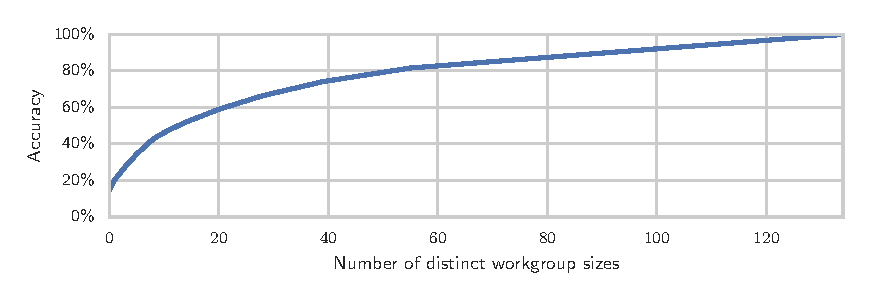
\includegraphics[width=\columnwidth]{img/num_params_oracle.pdf}
% \caption[Oracle accuracy vs.\ number of workgroup sizes]{%
%   Accuracy compared to the oracle as a function of the number of
%   workgroup sizes used. The best accuracy that can be achieved using a
%   single statically chosen workgroup size is 15\%. Achieving 50\%
%   oracle accuracy requires a minimum of 14 distinct workgroup sizes.%
% }
% \label{fig:oracle-accuracy}
% \end{figure}

The workgroup size optimisation space is non linear and
complex. Across the 429 different scenarios, there are 135 unique
oracle workgroup sizes, with 31.5\% of scenarios having a unique
workgroup size.
% Figure~\ref{fig:oracle-accuracy} plots the potential oracle accuracy
% as a function of the number of workgroup sizes.
The average speedup of the oracle workgroup size over the worst
workgroup size for each scenario is $15.14\times$ (min $1.03\times$,
max
$207.72\times$). % Figure~\ref{fig:performances} plots the performance
% of workgroup sizes relative to the oracle for all test cases,
% demonstrating both the profit XXX optimisation space, and the uneven
% XXX response to XXX.

% \begin{figure}
%   \begin{subfigure}[h]{\columnwidth}
%     \centering
%     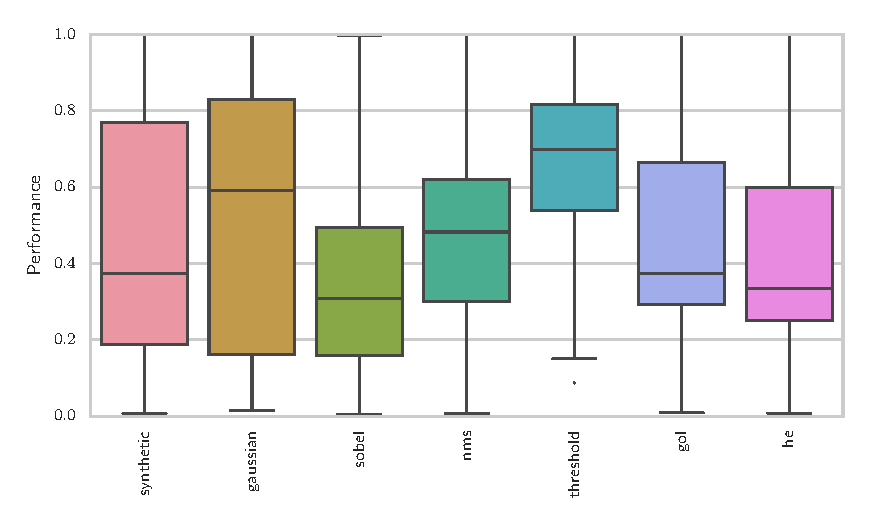
\includegraphics[width=\columnwidth]{img/performance_kernels.pdf}
%     \vspace{-1.5em} % Shrink vertical padding
%     \caption{}
%     \label{fig:performance-kernels}
%   \end{subfigure}
%   \\
%   \begin{subfigure}[h]{.48\columnwidth}
%     \centering
%     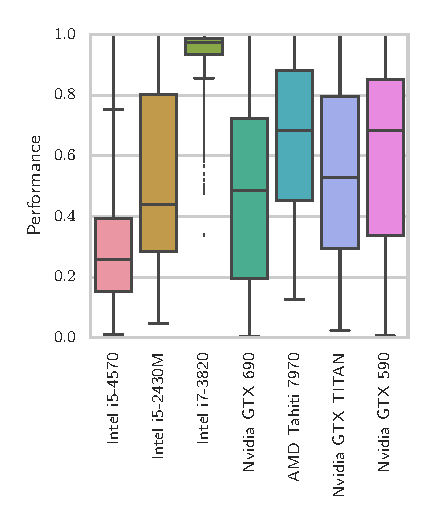
\includegraphics[width=\columnwidth]{img/performance_devices.pdf}
%     \vspace{-1.5em} % Shrink vertical padding
%     \caption{}
%     \label{fig:performance-devices}
%   \end{subfigure}
%   ~%
%   \begin{subfigure}[h]{.48\columnwidth}
%     \centering
%     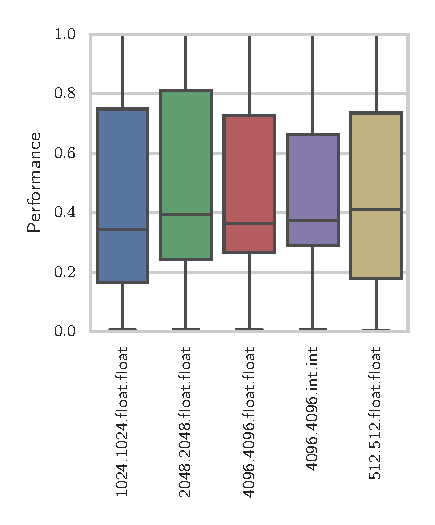
\includegraphics[width=\columnwidth]{img/performance_datasets.pdf}
%     \vspace{-1.5em} % Shrink vertical padding
%     \caption{}
%     \label{fig:performance-datasets}
%   \end{subfigure}
%   \caption[Workgroup size performances across device, kernel, and dataset]{%
%     Performance relative to the oracle of workgroup sizes across all
%     test cases, grouped by: (\subref{fig:performance-kernels})~kernels,
%     (\subref{fig:performance-devices})~devices, and
%     (\subref{fig:performance-datasets})~datasets.%
%   }
% \label{fig:performances}
% \end{figure}

% Note too that for 5 of the scenarios, the speedup of the best over
% worst workgroup sizes is $\le 5\%$. For these scenarios, there is
% little benefit to autotuning; however, this represents only 1.1\% of
% the tested scenarios. For 50\% of the scenarios, the speedup of the
% best over worst workgroup sizes is $\ge 6.19\times$.

Of the 8504 unique workgroup sizes tested, 11.4\% were refused in one
or more test cases, with an average of 5.5\% test cases leading to
refused parameters. While there are certain patterns (for example,
workgroup sizes which contain $w_c$ and $w_r$ values which are
multiples of eight are less frequently refused, which is a common
width of SIMD vector operations~\cite{IntelCorporation2012}), a
refused parameter is an obvious inconvenience to the user, as one
would expect that any workgroup size within the specified maximum
should behave \emph{correctly}, if not efficiently.

\begin{figure}
  \centering
  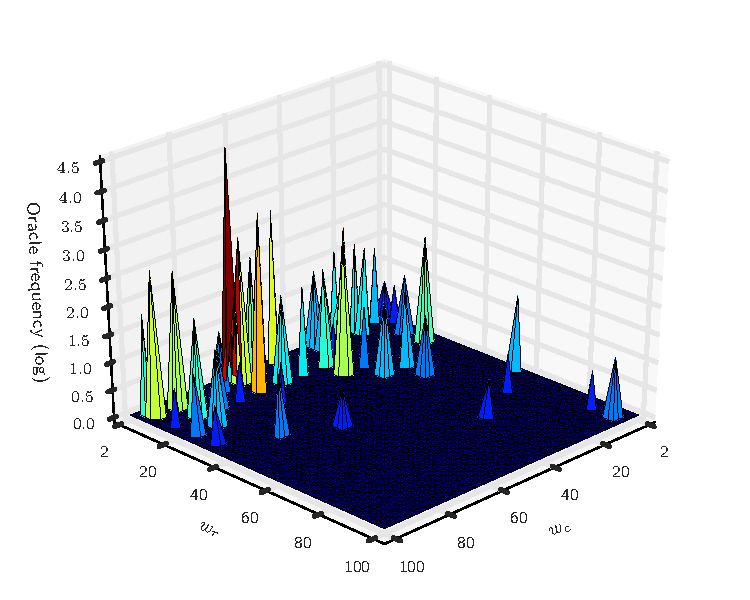
\includegraphics[width=\columnwidth]{img/oracle_param_space.pdf}
  \caption{%
    Oracle frequency counts for a subset of the workgroup sizes,
    $w_c \le 100, w_r \le 100$. The most commonly optimal workgroup
    size is $w_{(64 \times 4)}$, accounting for 15\% of test cases. 14
    distinct workgroup sizes account for 50\% of the oracle workgroup
    sizes.%
  }
\label{fig:oracle-wgsizes}
\end{figure}

\begin{figure}
  \centering
  \centering
  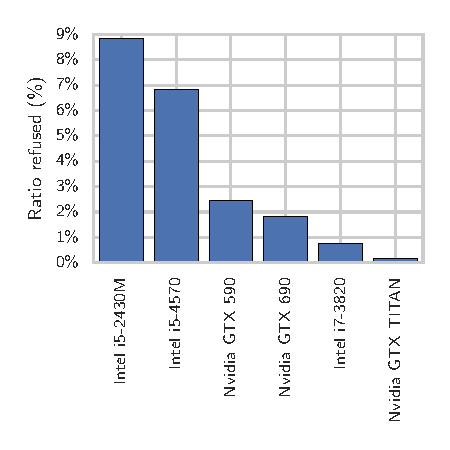
\includegraphics[width=.75\columnwidth]{img/refused_params_by_device}
  \caption[Refused workgroup sizes by device and vendor]{%
    The ratio of test cases with refused workgroup sizes, grouped by
    OpenCL device ID. No parameters were refused by AMD devices.%
  }
\label{fig:refused-params}
\end{figure}

Experimental results suggest that the problem is vendor --- or at
least device --- specific. Figure~\ref{fig:refused-params} shows the
ratio of refused test cases, grouped by device. We see a much greater
quantity of refused parameters for test cases on Intel CPU devices
than any other type, while no workgroup sizes were refused by the AMD
GPU. The exact underlying cause for these refused parameters is
unknown, but can likely by explained by inconsistencies or errors in
specific OpenCL driver implementations. As these OpenCL
implementations are still in active development, it is anticipated
that errors caused by unexpected behaviour will become more infrequent
as the technology matures. Note that the ratio of refused parameters
decreases across the three generations of Nvidia GPUs: GTX 590 (2011),
GTX 690 (2012), and GTX TITAN (2013). For now, it is imperative that
any autotuning system is capable of adapting to these refused
parameters by suggesting alternatives when they occur.

The baseline parameter $\bar{w}$ is the workgroup size which provides
the best overall performance while being legal for all
scenarios. Because of refused parameters, only a \emph{single}
workgroup size $w_{(4 \times 4)}$ from the set of experimental results
is found to have a legality of 100\%, suggesting that an adaptive
approach to setting workgroup size is necessary not just for the sake
of maximising performance, but also for guaranteeing program
correctness. The utility of the baseline parameter is that it
represents the best performance that can be achieved through static
tuning of the workgroup size parameter. We can evaluate the
performance of suboptimal workgroup sizes by calculating the geometric
mean of their \emph{performance} for a particular scenario $p(s, w)$
across all scenarios, $\bar{p}(w)$. The baseline parameter
$\bar{p}(\bar{w})$ achieves only 24\% of the available performance.


\section{Evaluation}

In this section we evaluate the effectiveness of the three proposed
autotuning techniques. For each autotuning technique, we partition the
experimental data into training and testing sets. Three strategies for
partitioning the data are used: the first is a 10-fold
cross-validation; the second is to divide the data such that only data
collected from synthetic benchmarks are used for training and only
data collected from the real-world benchmarks are used for testing;
the third approach is to create leave-one-out partitions for each
unique device, kernel, and dataset. Then, for each combination of
autotuning technique and training data, we evaluate each of the
workgroup sizes predicted for the testing data using the following
metrics:
%
\begin{itemize}
\item time (real) --- the time taken to make the autotuning
  prediction. This includes classification time and any communication
  overheads.
\item accuracy (binary) --- whether the predicted workgroup size is
  the true oracle, $w = \Omega(s)$.
\item validity (binary) --- whether the predicted workgroup size
  satisfies the workgroup size constraints constraints,
  $w < W_{\max}(s)$.
\item refused (binary) --- whether the predicted workgroup size which
  is refused, $w \in W_{refused}(s)$.
\item performance (real) --- the relative performance of the predicted
  workgroup size relative to the oracle.
  % $0 \le \frac{t(s,\Omega(s))}{t(s,w)} \le 1$.
\item speedups (real) --- the relative performance of the predicted
  workgroup size relative to the baseline workgroup size
  $w_{(4 \times 4)}$, and human expert workgroup size
  $w_{(32 \times 4)}$ (where applicable).
\end{itemize}
%
The \emph{validty} and \emph{refused} metrics measure how often
fallback strategies are required to select a legal workgroup size
$w \in W_{legal}(s)$. This is only required for the classification
approach to autotuning, since the process of selecting workgroup sizes
using regressors respects workgroup size constraints.

\begin{figure}
\centering
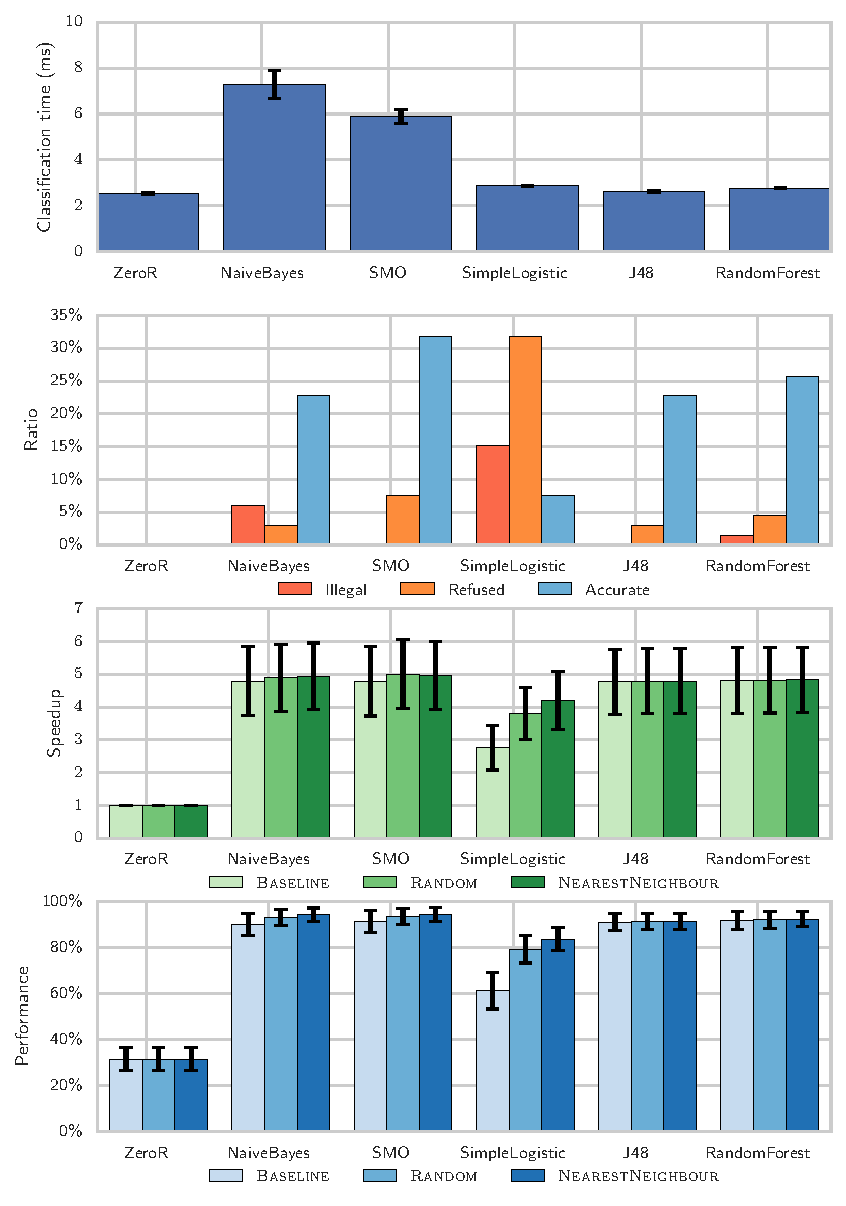
\includegraphics[width=\columnwidth]{img/classification-syn-real}
\caption[Classification results using synthetic benchmarks]{%
  Autotuning results using classifiers and synthetic benchmarks. Each
  classifier is trained on data collected from synthetic stencil
  applications, and tested for prediction quality using data from 6
  real-world benchmarks. Each of the different values correspond to a
  different data partitioning strategy, e.g.\ cross-kernel
  partitioning, 10-fold validation, etc.%
}
\label{fig:class-syn}
\end{figure}

% \begin{figure}
% \centering
% 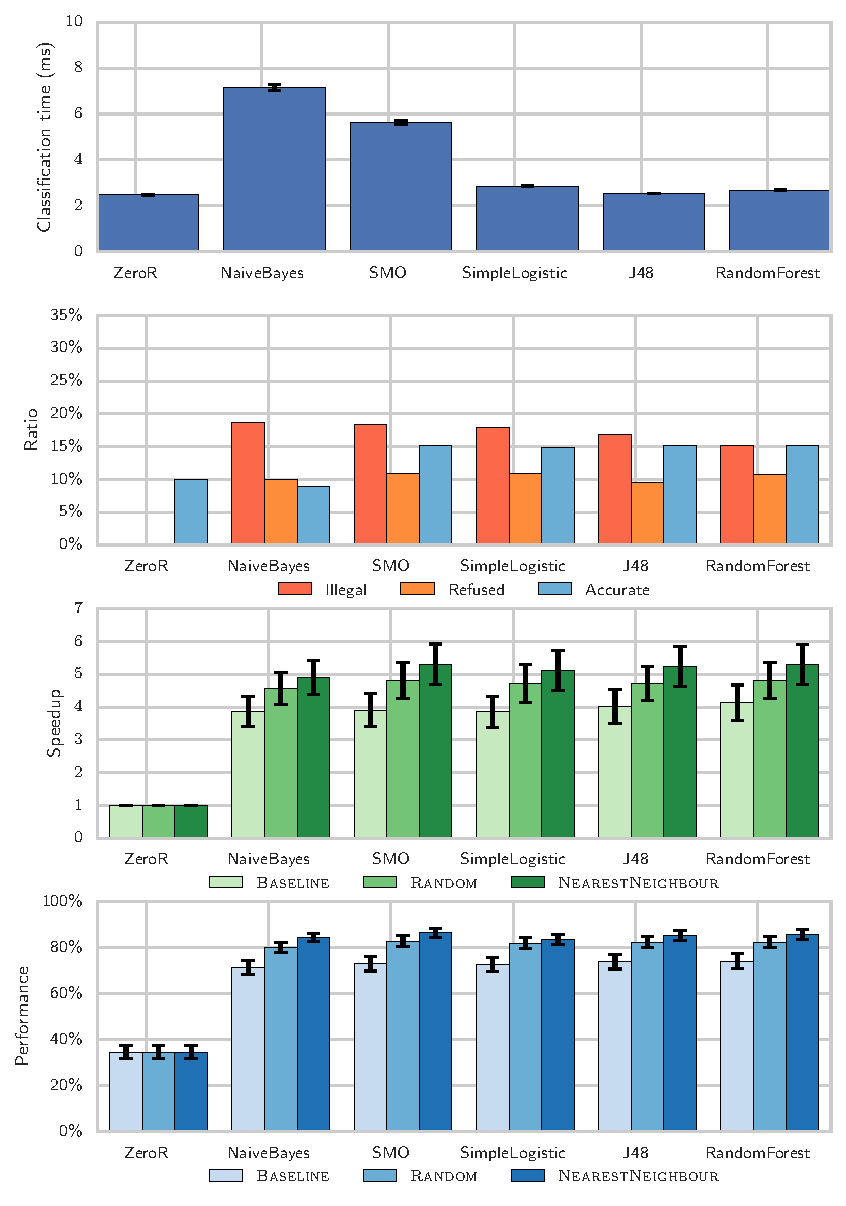
\includegraphics[width=\columnwidth]{img/classification-arch}
% \caption[Classification results using cross-device evaluation]{%
%   Classification results of cross-device evaluation. Each classifier
%   is trained using data from $n-1$ devices, and tested for prediction
%   quality using data for the $n^{th}$ device.%
% }
% \label{fig:class-arch}
% \end{figure}

\begin{figure}
\centering
\begin{subfigure}[h]{.48\columnwidth}
\centering
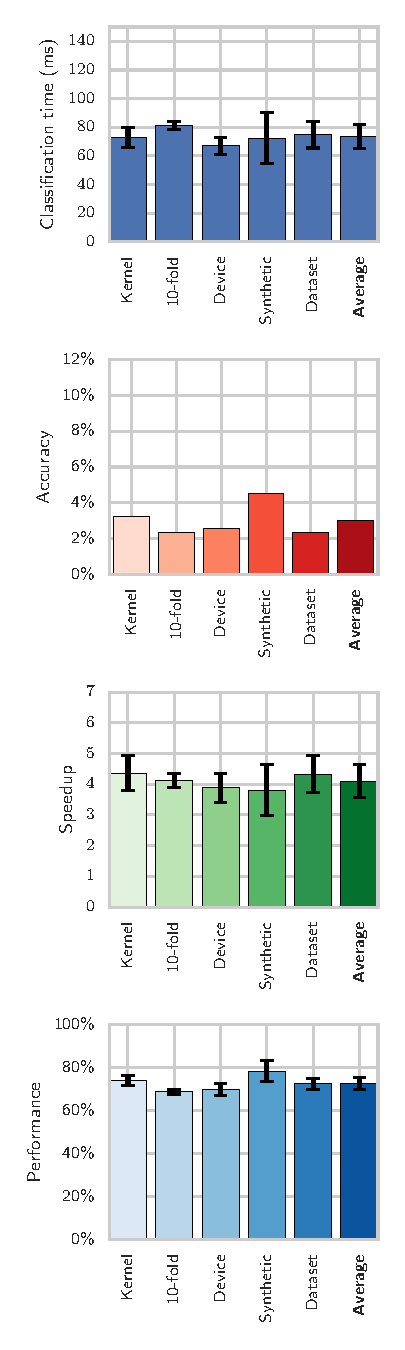
\includegraphics[width=\columnwidth]{img/runtime-class-xval}
\caption{}
\label{fig:runtime-class-xval}
\end{subfigure}
\begin{subfigure}[h]{.48\columnwidth}
\centering
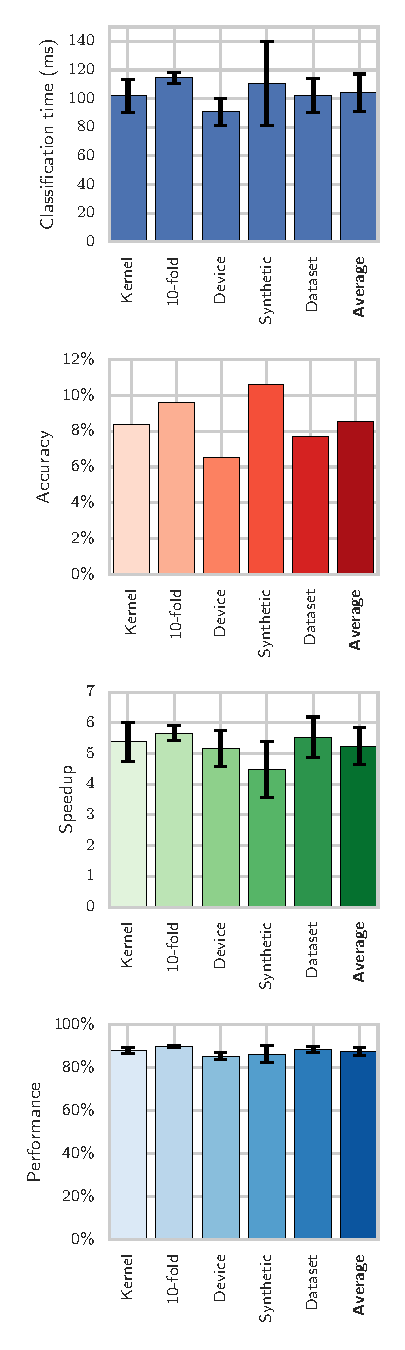
\includegraphics[width=\columnwidth]{img/speedup-class-xval}
\caption{}
\label{fig:speedup-class-xval}
\end{subfigure}
\caption[Autotuning performance using regressors]{%
  Autotuning results using regressors which predict:
  (\subref{fig:runtime-class-xval}) the workgroup size with the
  minimal runtime, and (\subref{fig:speedup-class-xval}) the workgroup
  size with the greatest speedup over a baseline.%
}
\label{fig:regression-class}
\end{figure}

\subsection{Autotuning with Classifiers}

With the exception of the ZeroR, which predicts \emph{only} the
baseline workgroup size $w_{\left( 4 \times 4 \right)}$, the
classifiers achieve good speedups over the baseline, ranging from
$4.61\times$ to $5.05\times$ when averaged across all partitioning
strategies. Figure~\ref{fig:class-syn} shows the results when
classifiers are trained using data from synthetic benchmarks and
tested using real-world benchmarks. The highest average speedup is
achieved by the SMO classifier, and the lowest by Naive Bayes. The
difference between average speedups is not significant between the
types of classifier, with the exception of SimpleLogistic, which
performs poorly when trained with synthetic benchmarks and tested
against real-world programs. This suggests the model over-fitting to
features of the synthetic benchmarks which are not shared by the
real-world tests.

Of the three approaches to handling invalid predictions, the fallback
handler with the best average case performance is
\textsc{NearestNeighbour}, achieving an average speedup across all
classifiers and validation sets of $5.26\times$. The speedup of
\textsc{Random} fallback handler is $3.69\times$, and $1.0\times$ for
\textsc{Baseline}. Interestingly, both the lowest and highest speedups
are achieved by the \textsc{Random} fallback handler, since it
essentially performs a random exploration of the optimisation
space. However, the \textsc{NearestNeighbour} fallback handler
provides consistently greater speedups for the majority of test cases,
indicating that it successfully exploits structure in the optimisation
spaces.


\subsection{Autotuning with Regressors}

Figures~\ref{fig:runtime-class-xval} and ~\ref{fig:speedup-class-xval}
show a summary of results for classification using regressors to
predict program runtimes and speedups, respectively. Of the two
regression techniques, predicting the \emph{speedup} of workgroup
sizes is much more successful than predicting the \emph{runtime}. This
is most likely caused by the inherent difficulty in predicting the
runtime of arbitrary code, where dynamic factors such as flow control
and loop bounds are not captured by static instruction counts and
densities which are used as features by the machine learning
models. The average speedup achieved by predicting runtimes is
$4.14\times$. For predicting speedups, the average is $5.57\times$.

The prediction costs using regression are significantly greater than
using classifiers. This is because, while a classifier makes a single
prediction, the number of predictions required of a regressor grows
with the size of $W_{\max}(s)$, since classification with regression
requires making predictions for all
$w \in \left\{ w | w < W_{\max}(s) \right\}$. The fastest classifier
is J48, due to the it's simplicity --- it can be implemented as a
sequence of nested \texttt{if} and \texttt{else} statements.


\subsection{Comparison with Human Expert}

\begin{figure}
\centering
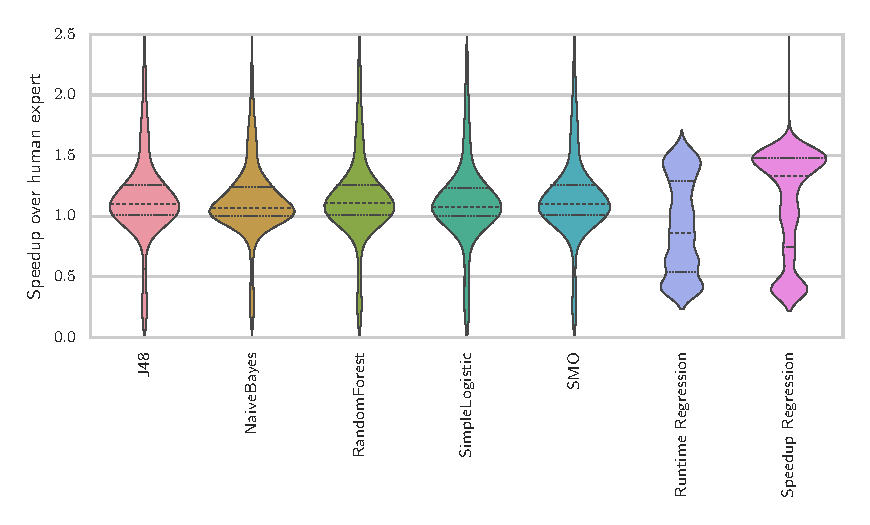
\includegraphics[width=\columnwidth]{img/speedup-distributions}
\caption[Speedup results over human expert]{%
  Distributions of speedups over \emph{human expert}, ignoring cases
  where human expert prediction is invalid. Classifiers are using
  \textsc{NearestNeighbour} fallback handlers. The speedup axis is
  fixed to the range 0--2.5 to highlight the IQRs, which results in
  some outliers > 2.5 being clipped.%
}
\label{fig:speedup-distributions}
\end{figure}

In the original implementation of the SkelCL stencil
skeleton~\cite{Breuer2014a}, \citeauthor{Breuer2014a} selected a
workgroup size of $w_{(32 \times 4)}$ in an evaluation of 4 stencil
operations on a Tesla S1070 system. In our evaluation of 429
combinations of kernel, architecture, and dataset, we found that this
workgroup size is refused by 2.6\% of scenarios, making it unsuitable
for use as a baseline. However, if we remove the scenarios for which
$w_{(32 \times 4)}$ is \emph{not} a legal workgroup size, we can use
this as an additional workgroup size to compare the relative
performance of predictions against.

Figure~\ref{fig:speedup-distributions} plots the distribution of
speedups for all test instances over the human expert parameter, for
each autotuning technique. The speedup distributions show consistent
classification results for the five classification techniques, with
the speedup at the lower quartile for all classifiers being
$\ge 1.0\times$. The IQR for all classifiers is $< 0.5$, but there are
outliers with speedups both well below $1.0\times$ and well above
$2.0\times$. In contrast, the speedups achieved using regressors to
predict runtimes have a lower range, but also a lower median and a
larger IQR. Clearly, this approach is the least effective of the
evaluated autotuning techniques. Using regressors to predict relative
performance is more successful, with the highest median speedup of all
the techniques. However, it also has a large IQR and the lower
quartile has a speedup value well below 1, meaning that for more than
25\% of test instances, the workgroup size selected did not perform as
well as the human expert selected workgroup size.


% \begin{figure}
% \centering
% \begin{subfigure}[t]{0.48\columnwidth}
% \centering
% 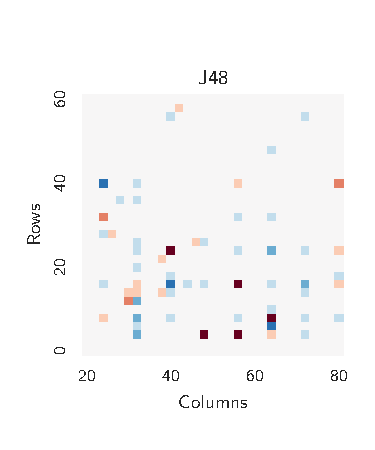
\includegraphics[width=\columnwidth]{img/heatmap_1}
% \vspace{-1.5em} % Shrink vertical padding
% \caption{}
% \label{fig:class-hmaps-1}
% \end{subfigure}
% \begin{subfigure}[t]{0.48\columnwidth}
% \centering
% 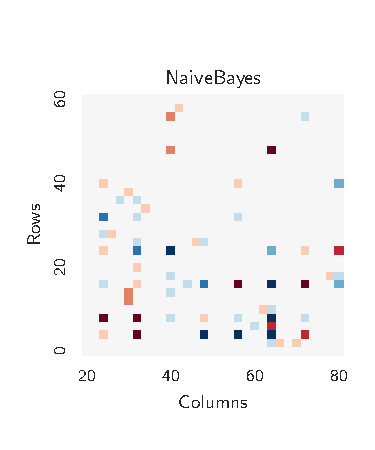
\includegraphics[width=\columnwidth]{img/heatmap_2}
% \vspace{-1.5em} % Shrink vertical padding
% \caption{}
% \label{fig:class-hmaps-2}
% \end{subfigure}
% \\
% \begin{subfigure}[t]{0.48\columnwidth}
% \centering
% 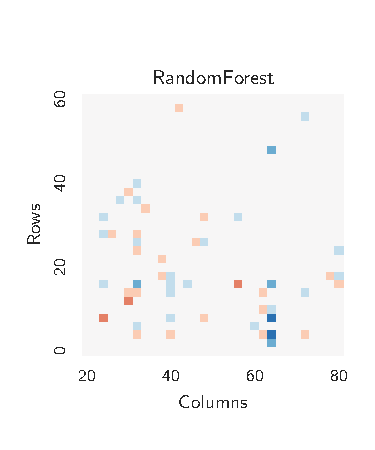
\includegraphics[width=\columnwidth]{img/heatmap_3}
% \vspace{-1.5em} % Shrink vertical padding
% \caption{}
% \label{fig:class-hmaps-3}
% \end{subfigure}
% \begin{subfigure}[t]{0.48\columnwidth}
% \centering
% 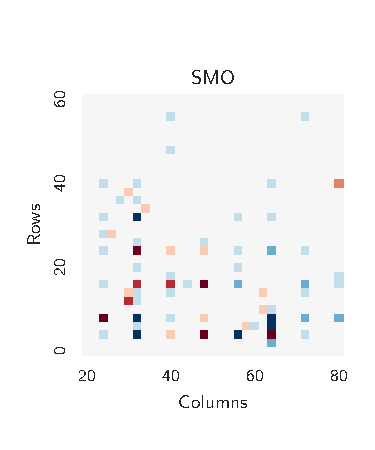
\includegraphics[width=\columnwidth]{img/heatmap_5}
% \vspace{-1.5em} % Shrink vertical padding
% \caption{}
% \label{fig:class-hmaps-4}
% \end{subfigure}
% \\
% \begin{subfigure}[t]{0.48\columnwidth}
% \centering
% 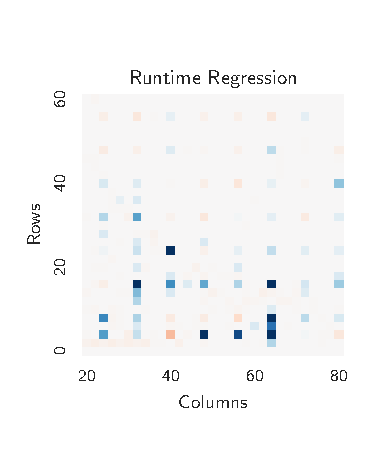
\includegraphics[width=\columnwidth]{img/reg_runtime_heatmap}
% \vspace{-1.5em} % Shrink vertical padding
% \caption{}
% \label{fig:class-hmaps-5}
% \end{subfigure}
% \begin{subfigure}[t]{0.48\columnwidth}
% \centering
% 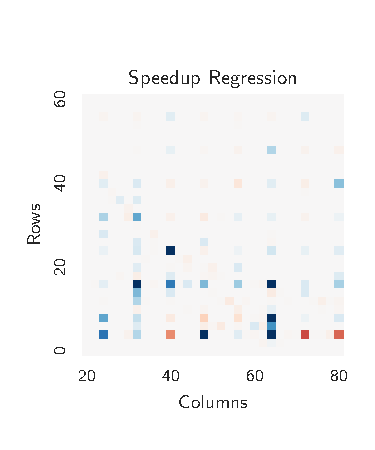
\includegraphics[width=\columnwidth]{img/reg_speedup_heatmap}
% \vspace{-1.5em} % Shrink vertical padding
% \caption{}
% \label{fig:class-hmaps-6}
% \end{subfigure}
% \caption[Classification error heatmaps]{%
%   Heatmaps of classification errors for 10-fold cross-validation,
%   showing a subset of the optimisation space. The shading in each
%   cells indicates if it is predicted less frequently (blue), ore more
%   frequently (red) than it is optimal. Colour gradients are normalised
%   across plots.%
% }
% \label{fig:class-hmaps}
% \end{figure}

% Figure~\ref{fig:class-hmaps} visualises the classification errors of
% each of the autotuning techniques. It shows that while the performance
% of all of the classifiers is comparable, the distribution of
% predictions is not. Only the NaiveBayes and RandomForest classifiers
% predicted the human expert selected workgroup size of
% $w_{(32 \times 4)}$ as frequently, or more frequently, than it was
% optimal. The two regression techniques were the least accurate of all
% of the autotuning techniques.


\section{Related Work}\label{sec:related}

% Iterative compilation is the method of performance tuning in which a
% program is compiled and profiled using multiple different
% configurations of optimisations in order to find the configuration
% which maximises performance. One of the the first formalised
% publications of the technique appeared in \citeyear{Bodin1998} by
% \citeauthor{Bodin1998}~\cite{Bodin1998}.  Iterative compilation has
% since been demonstrated to be a highly effective form of empirical
% performance tuning for selecting compiler optimisations.

% Given the huge number of possible compiler optimisations (there are
% 207 flags and parameters to control optimisations in GCC v4.9), it
% is often unfeasible to perform an exhaustive search of the entire
% optimisation space, leading to the development of methods for
% reducing the cost of evaluating configurations. These methods reduce
% evaluation costs either by shrinking the dimensionality or size of
% the optimisation space, or by guiding a directed search to traverse
% a subset of the space.

% Machine learning has been successful applied to this problem,
% in~\cite{Stephenson2003}, using ``meta optimisation'' to tune
% compiler heuristics through an evolutionary algorithm to automate
% the search of the optimisation space. \citeauthor{Fursin2011}
% continued this with Milepost GCC, the first machine learning-enabled
% self-tuning compiler~\cite{Fursin2011}. A recent survey of the use
% of machine learning to improve heuristics quality by
% \citeauthor{Burke2013} concludes that the automatic
% \emph{generation} of these self-tuning heuristics but is an ongoing
% research challenge that offers the greatest generalisation
% benefits~\cite{Burke2013}.

\citeauthor{Ganapathi2009} demonstrated early attempts at autotuning
multicore stencil codes in~\cite{Ganapathi2009}, presenting an
autotuner which evaluates a random 1500 selections from an space of 10
million optimisations, achieving 18\% better than that of a human
expert. The Kernel Canonical Correlation Analysis used in their
autotuner restricts the scalability of their system, as the complexity
of model building grows exponentially with the number of features. In
their evaluation, the system requires two hours of compute time to
build the model for only 400 seconds of benchmark data.

% \citeauthor{Berkeley2009} targeted 3D stencils code performance
% in~\cite{Berkeley2009}. Stencils are decomposed into core blocks,
% sufficiently small to avoid last level cache capacity misses. These
% are then further decomposed to thread blocks, designed to exploit
% common locality threads may have within a shared cache or local
% memory. Thread blocks are divided into register blocks in order to
% take advantage of data level parallelism provided by the available
% registers. Data allocation is optimised on NUMA systems. The
% performance evaluation considers speedups of various optimisations
% with and without consideration for host/device transfer overhead.

\citeauthor{Kamil2010} present an autotuning framework
in~\cite{Kamil2010} which accepts as input a Fortran 95 stencil
expression and generates tuned shared-memory parallel implementations
in Fortan, C, or CUDA. The system uses an IR to explore autotuning
transformations, enumerating a subset of the optimisation space and
recording only a single execution time for each configuration,
reporting the fastest. They demonstrate their system on 4
architectures using 3 benchmarks, with speedups of up to $22\times$
compared to serial implementations. The CUDA code generator does not
optimise for the GPU memory hierarchy, using only global memory. As
demonstrated in this work, improper utilisation of local memory can
hinder program performance by two orders of magnitude.
% There is no directed search or cross-program learning.

% In~\cite{Zhang2013a}, \citeauthor{Zhang2013a} present a code generator
% and autotuner for 3D Jacobi stencil codes. Using a DSL to express
% kernel functions, the code generator performs substitution from one of
% two CUDA templates to create programs for execution on GPUs. GPU
% programs are parameterised and tuned for block size, block dimensions,
% and whether input data is stored in read only texture memory. This
% creates an optimisation space of up to 200 configurations. In an
% evaluation of 4 benchmarks, the authors report impressive performance
% that is comparable with previous implementations of iterative Jacobi
% stencils on GPUs~\cite{Holewinski2012, Phillips2010}. The dominating
% parameter is shown to be block dimensions, followed by block size,
% then read only memory. The DSL presented in the paper is limited to
% expressing only Jacobi Stencils applications. Critically, their
% autotuner requires a full enumeration of the parameter space for each
% program. Since there is no indication of the compute time required to
% gather this data, it gives the impression that the system would be
% impractical for the needs of general purpose stencil computing. The
% autotuner presented in this thesis overcomes this drawback by learning
% parameter values which transfer to unseen stencils, without the need
% for an expensive tuning phase for each program and architecture.

% In~\cite{Christen2011}, \citeauthor{Christen2011} presentf a DSL for
% expressing stencil codes, a C code generator, and an autotuner for
% exploring the optimisation space of blocking and vectorisation
% strategies. The DSL supports stencil operations on arbitrarily
% high-dimensional grids. The autotuner performs either an exhaustive,
% multi-run Powell search, Nelder Mead, or evolutionary search to find
% optimal parameter values. They evaluate their system on two CPUS and
% one GPU using 6 benchmarks. A comparison of tuning results between
% different GPU architectures would have been welcome, as the results
% presented in this thesis show that devices have different responses to
% optimisation parameters. The authors do not present a ratio of the
% available performance that their system achieves, or how the
% performance of optimisations vary across benchmarks or devices.

PARTANS is an autotuning framework which targets the size of the halo
region for multi-GPU stencils~\cite{Lutz2013}. \citeauthor{Lutz2013}
explore the effect of varying the optimisation space using six
benchmark applications, finding that the optimal halo size depends on
the size of the grid, the number of partitions, and the connection
mechanism. The authors present an autotuner which determines problem
decomposition and swapping strategy offline, and performs an online
search for the optimal halo size. The selection of overlapping halo
region size compliments the selection of workgroup size which is the
subject of this thesis. However, PARTANS uses a custom DSL rather than
the generic interface provided by SkelCL, and PARTANS does not learn
the results of tuning across programs, or across multiple runs of the
same program.

\citeauthor{Collins2012} autotune Algorithmic Skeletons
in~\cite{Collins2012}, first using Principle Components Analysis to
reduce the dimensionality of the optimisation space, followed by a
search of parameter values to optimise program performance by a factor
of $1.6\times$ over values chosen by a human
expert. In~\cite{Collins2013}, they extend this using static feature
extraction and nearest neighbour classification to further prune the
search space, achieving an average 89\% of the oracle performance
after evaluating 45 parameters.

A method for the automatic generation of synthetic benchmarks for the
purpose of performance tuning is presented in~\cite{Chiu2015}, using
parameterised template substitution over a user-defined range of
values to generate training programs. The authors describe an
application of their tool for generating OpenCL stencil kernels, but
do not report any performance results.

% Performant GPGPU programs require careful attention from the developer
% to properly manage data layout in DRAM, caching, diverging control
% flow, and thread communication. The importance of proper exploitation
% of local shared memory and synchronisation costs is explored
% in~\cite{Lee2010}. In~\cite{Chen2014}, data locality optimisations are
% automated using a description of the hardware and a
% memory-placement-agnostic compiler. The authors demonstrate impressive
% speedups of up to $2.08\times$, although at the cost of requiring
% accurate memory hierarchy descriptor files for all targeted
% hardware. The descriptor files must be hand generated, requiring
% expert knowledge of the underlying hardware in order to properly
% exploit memory locality.


\section{Conclusions}\label{sec:conclusions}

In this paper we propose three methodologies for autotuning workgroup
size of OpenCL stencil kernels. We evaluate the effectiveness of each
approach in a large empirical performance comparison of 429
combinations of architecture, kernel, and dataset, measuring an
average of 629 different workgroup sizes for each scenario. We find
that the performance gap between the best and worst workgroup size is
up to $207.72\times$. Differing scenarios have wildly different
optimal workgroup sizes, and only 24\% of the available performance
can be achieved using static tuning.

From an evaluation of 17 different autotuning techniques using 5
different types of validation sets, the following conclusions about
autotuning performance can be drawn:
%
\begin{itemize}
\item In the case of classifiers predicting illegal workgroup sizes,
  the best fallback strategy is to select the closest legal workgroup
  size.
\item The performance of predicted workgroup sizes for unseen devices
  is within 8\% of the performance for known devices.
\item Predicting the \emph{runtime} of stencils is the least effective
  of the evaluated autotuning techniques, achieving an average of only
  68\% of the available performance.
\item Predicting the \emph{speedup} of workgroup sizes provides the
  highest median speedup, but more frequently predicts a poorly
  performing workgroup size then the classifiers.
\item Classification using regression costs an order of magnitude more
  time than using classifiers. The J48 classifier has the lowest
  overhead.
\end{itemize}

% In this thesis, I have presented my attempt at providing such a
% system, by designing a novel framework which has the benefits of fast,
% ``always-on'' autotuning, while being able to synchronise data with
% global repositories of knowledge which others may contribute to. The
% framework provides an interface for autotuning which is sufficiently
% generic to be easily re-purposed to target a range of optimisation
% parameters.

% To demonstrate the utility of this framework, I implemented a frontend
% for predicting the workgroup size of OpenCL kernels for SkelCL stencil
% codes. This optimisation space is complex, non linear, and critical
% for the performance of stencil kernels, with up to a $207.72\times$
% slowdown if an improper value is picked. Selecting the correct
% workgroup size is difficult --- requiring a knowledge of the kernel,
% dataset, and underlying architecture. The challenge is increased even
% more so by inconsistencies in the underlying system which cause some
% workgroup sizes to fail completely. Of the 269813 combinations of
% workgroup size, device, program, and dataset tested; only a
% \emph{single} workgroup size was valid for all test cases, and
% achieved only 24\% of the available performance. The value selected by
% human experts was invalid for 2.6\% of test cases. Autotuning in this
% space requires a system which is resilient these challenges, and
% several techniques were implemented to address them.

% Runtime performance of autotuned stencil kernels is very promising,
% achieving an average 90\% of the available performance with only a 3ms
% autotuning overhead. Even ignoring the cases for which the human
% expert selected workgroup size is invalid, this provides a
% $1.33\times$ speedup, or a $5.57\times$ speedup over the best
% performance that can be achieved using static tuning. Classification
% performance is comparable when predicting workgroup sizes for both
% unseen programs and unseen devices. I believe that the combination of
% performance improvements and the collaborative nature of OmniTune
% makes for a compelling case for the use of autotuning as a key
% component for enabling performant, high level parallel programming.


% \subsection{Critical Analysis}

% This subsection contains a critical analysis of the work presented in
% previous sections.

% \paragraph{OmniTune Framework}

% The purpose of the OmniTune framework is to provide a generic
% interface for runtime autotuning. This is demonstrated through the
% implementation of a SkelCL frontend; however, to truly evaluate the
% ease of use of this framework, it would have been preferable to
% implement one or more additional autotuning frontends, to target
% different optimisation spaces. This could expose any leakages in the
% abstractions between the SkelCL-specific and generic autotuning
% components.


% \paragraph{Synthetic Benchmarks}

% The OmniTune SkelCL frontend provides a template substitution engine
% for generating synthetic stencil benchmarks. The implementation of
% this generator is rigidly tied to the SkelCL stencil format. It would
% be preferred if this template engine was made more flexible, to
% support generation of arbitrary test programs. Additionally, due to
% time constraints, I did not have the opportunity to explore how the
% number of synthetic benchmarks in machine learning test data sets
% affects classification performance.

% One possible use of the synthetic stencil benchmark generator could be
% for creating minimal test cases of refused OpenCL parameters so that
% bug reports could be filed with the relevant implementation
% vendor. However, this would have added a great level of complexity to
% the the generator, as it would have to isolate and remove the
% dependency on SkelCL to generate minimal programs, requiring
% significant implementation work.


% \paragraph{Use of Machine Learning}

% The evaluation of OmniTune in this thesis uses multiple classifiers
% and regressors to predict workgroup sizes. The behaviour of these
% classifiers and regressors is provided by the Weka data mining
% suite. Many of these classifiers have parameters which affect their
% prediction behaviour. The quality of the evaluation could have been
% improved by exploring the effects that changing the values of these
% parameters has on the OmniTune classification performance. It would
% also have been informative to dedicate a portion of the evaluation to
% feature engineering, evaluating the information gain of each feature
% and exploring the effects of feature transformations on classification
% performance.


% \paragraph{Evaluation Methodology}

% The evaluation compares autotuning performance against the best
% possible performance that can be achieved using static tuning, a
% simple heuristic to tune workgroup size on a per-device basis, and
% against the workgroup size chosen by human experts. It would have been
% beneficial to also include a comparison of the performance of these
% autotuned stencils against hand-crafted equivalent programs in pure
% OpenCL, without using the SkelCL framework. This would allow a direct
% comparison between the performance of stencil kernels using high level
% and low level abstractions, but could not be completed due to time
% constraints and difficulties in acquiring suitable comparison
% benchmarks and datasets.


% \subsection{Future Work}

% Future work can be divided into two categories: continued development
% of OmniTune, and extending the behaviour of the SkelCL autotuner.

% The cost of offline training with OmniTune could be reduced by
% exploring the use of adaptive sampling plans, such as presented
% in~\cite{Leather2009}. This could reduce the number of runtime samples
% required to distinguish good from bad optimisation parameter values.

% Algorithm~\ref{alg:autotune-hybrid} proposes the behaviour of a hybrid
% approach to selecting the workgroup size of iterative SkelCL
% stencils. This approach attempts to exploit the advantages of all of
% the techniques presented in this thesis. First, runtime regression is
% used to predict the minimum runtime and a candidate workgroup
% size. If, after evaluating this workgroup size, the predicted runtime
% turned out to be inaccurate, then a prediction is made using speedup
% regression. Such a hybrid approach would enable online tuning through
% the continued acquisition of runtime and speedup performance, which
% would compliment the collaborative aspirations of OmniTune, and the
% existing server-remote infrastructure.

% Other skeleton optimisation parameters could be autotuned by SkelCL,
% including higher level optimisations such as the selection of border
% region loading strategy, or selecting the optimal execution device(s)
% for multi-device systems. Optimisation parameters of additional
% skeletons could be autotuned, or the interaction of multiple related
% optimisation parameters could be explored. Power consumption could be
% used as an additional optimisation cotarget.

% \begin{algorithm}
% \begin{algorithmic}[1]
% \Require kernel features $k$, hardware features $h$, dataset features $d$.
% \Ensure workgroup size $w$

% \State $r \leftarrow \underset{w \in W_{legal}(s)}{\min} f(k,h,d,w)$
% \Comment Predict minimum runtime.
% \State $w \leftarrow \underset{w \in W_{legal}(s)}{\argmin} f(k,h,d,w)$
% \Comment Workgroup size for $r$.
% \State $t_r \leftarrow$ measure runtime of program with $w$
% \State \textsc{Submit}$\left( f(s), w, t_r \right)$
% \Comment Submit observed runtime
% \If{$t_r \approx r$}
% \State \textbf{return} $w$
% \Comment Predicted runtime is accurate.
% \Else
% \State $W \leftarrow \left\{ w | w < W_{\max}(s) \right\}$
% \State converged $\leftarrow$ false
% \State $w_b \leftarrow$ baseline parameter
% \State $t_b \leftarrow$ measure runtime of runtime of program with
% $w_b$
% \State \textsc{Submit}$\left( f(s), w_b, t_b \right)$
% \Comment Submit observed runtime
% \While{not converged}
% \State $s \leftarrow \underset{w \in W}{\max} g(k,h,d,w)$
% \Comment Predict best speedup.
% \State $w \leftarrow \underset{w \in W}{\argmax} g(k,h,d,w)$
% \Comment Workgroup size for $s$.
% \State $t \leftarrow$ measure runtime of program with $s$
% \State \textsc{Submit}$\left( f(s), w, t \right)$
% \Comment Submit observed runtime
% \State $s_w \leftarrow t_t / t$
% \State \textsc{Submit}$\left( f(s), w, s_w \right)$
% \Comment Submit observed speedup
% \If{$s_w \approx s$}
% \State converged = true
% \Comment Predicted speedup is accurate.
% \Else
% \State $W = W - \{ w \}$
% \EndIf
% \EndWhile
% \State \textbf{return} $w$
% \EndIf
% \end{algorithmic}
% \caption{%
% Selecting workgroup size using a combination of classifiers and
% regressors.%
% }
%   \label{alg:autotune-hybrid}
% \end{algorithm}




\acks

This work was supported by grant EP/L01503X/1 for the University of
Edinburgh School of Informatics Centre for Doctoral Training in
Pervasive Parallelism
(\url{http://pervasiveparallelism.inf.ed.ac.uk/}) from the UK
Engineering and Physical Sciences Research Council (EPSRC).

% We recommend abbrvnat bibliography style.

\label{bibliography}
\printbibliography


\end{document}
